%%%%%%%%%%%%%%%%%%%%%%%%%%%%%%%%%%%%%%%%%
% Dreuw & Deselaer's Poster
% LaTeX Template
% Version 1.0 (11/04/13)
%
% Created by:
% Philippe Dreuw and Thomas Deselaers
% http://www-i6.informatik.rwth-aachen.de/~dreuw/latexbeamerposter.php
%
% This template has been downloaded from:
% http://www.LaTeXTemplates.com
%
% License:
% CC BY-NC-SA 3.0 (http://creativecommons.org/licenses/by-nc-sa/3.0/)
%
%%%%%%%%%%%%%%%%%%%%%%%%%%%%%%%%%%%%%%%%%

%----------------------------------------------------------------------------------------
%	PACKAGES AND OTHER DOCUMENT CONFIGURATIONS
%----------------------------------------------------------------------------------------

\documentclass[final,hyperref={pdfpagelabels=false}]{beamer}

\usepackage[orientation=portrait,size=a4,scale=1.3]{beamerposter} % Use the beamerposter package for laying out the poster with a portrait orientation and an a0 paper size

\usetheme{I6pd2} % Use the I6pd2 theme supplied with this template

\usepackage[english]{babel} % English language/hyphenation

\usepackage{amsmath,amsthm,amssymb,latexsym} % For including math equations, theorems, symbols, etc

%\usepackage{times}\usefonttheme{professionalfonts}  % Uncomment to use Times as the main font
%\usefonttheme[onlymath]{serif} % Uncomment to use a Serif font within math environments

\boldmath % Use bold for everything within the math environment

\usepackage{booktabs} % Top and bottom rules for tables

\graphicspath{{figures/}} % Location of the graphics files

\usecaptiontemplate{\small\structure{\insertcaptionname~\insertcaptionnumber: }\insertcaption} % A fix for figure numbering

%----------------------------------------------------------------------------------------
%	TITLE SECTION 
%----------------------------------------------------------------------------------------

\title{\huge YOLOv7 Small Object Detection Optimization to Detect Airborne Objects} % Poster title

\author[Dion Solang]{ 
  \parbox[t]{7cm}{
    \textbf{Author}\\
    Dion Andreas Solang\\
    NRP 07211940000039
  }
  \parbox[t]{7cm}{
    \textbf{Advisors}\\
    Reza Fuad Rachmadi, S.T., M.T., Ph.D\\
    Dr. I Ketut Eddy Purnama S.T., M.T.
  }
} % Author(s)

\institute{
  Department of Computer Engineering\\
  Institut Teknologi Sepuluh Nopember} % Institution(s)

%----------------------------------------------------------------------------------------
%	FOOTER TEXT
%----------------------------------------------------------------------------------------

\newcommand{\leftfoot}{messier12.github.io/yolov7ta} % Left footer text

\newcommand{\rightfoot}{solang.dion@gmail.com} % Right footer text

%----------------------------------------------------------------------------------------

\begin{document}

\addtobeamertemplate{block end}{}{\vspace*{2ex}} % White space under blocks

\begin{frame}[t] % The whole poster is enclosed in one beamer frame

\begin{block}{ABSTRACT}
  In this research, we present an attempt to improve the detection capability of YOLOv7 for airborne objects. 
  Airborne objects appear considerably small in camera images when they are located at a considerable distance from the camera. 
  However, due to their high speed of movement, it is crucial to detect them while they are still far away. 
  Therefore, to effectively detect these objects, YOLOv7 needs to be optimized for small objects.
  To address this challenge, we proposed several modifications that include changes in the architecture (adding an extra detection head, modifying the feature-map source, and replacing the detection head with a detached anchor-free head), application of bag-of-freebies techniques (anchor recalculation and mosaic augmentation), and change in the inference process (partitioning the image and performing inference on each partition).
  Through comprehensive experimentation, we have discovered that the combination of replacing the detection head with a detached anchor-free head, and performing inference on partitions yields the most promising results, with a significant increase in mean average precision (mAP) of 46.18\% while still maintaining real-time inference speed (greater than 10 FPS).
  This improvement is notably higher compared to the unmodified plain YOLOv7, which achieved a mAP score of 0\%.
  %Airborne objects appear very small on cameras.
  %YOLOv7 is the state of the art real-time object detector optimized for general object detections.
  %Thus, to detect airborne objects with YOLOv7, modifications are needed to be applied.
  %The purpose of this research is to find a modification solution for YOLOv7 to optimize its small object detection capability especially for airborne objects.
  %Modifications to be applied on YOLOv7 consists of architecture modifications and bag-of-freebies modifications.
  %Architecture modifications consist of neck modification and head layer addition.
  %Bag-of-freebies modifications consist of mosaic data augmentation dan active anchor recalculation.
  %These modifications will be combined one with another and have their performance tested.
  %Modifications that produces model with the highest mAP score on airborne objects dataset will be chosen as the optimization solution of this research.
\end{block}

\begin{columns}[t] % The whole poster consists of two major columns, each of which can be subdivided further with another \begin{columns} block - the [t] argument aligns each column's content to the top

\begin{column}{.02\textwidth}\end{column} % Empty spacer column

\begin{column}{.465\textwidth} % The first column

%----------------------------------------------------------------------------------------
%	OBJECTIVES
%----------------------------------------------------------------------------------------

\begin{block}{Objective}
  The objective of this research is to find modifications that can be made to YOLOv7
  such that it could detect airborne objects better.
\end{block}

%----------------------------------------------------------------------------------------
%	INTRODUCTION
%----------------------------------------------------------------------------------------
            
\begin{block}{Introduction}
  One of the greatest challenge in autonomous flight
  is about the problem of sensing and avoiding (SAA) airborne objects like bird, airplane, helicopter, and other.
  Camera is a popular choice of sensor for this task due to its cheaper price and small payload.
  One problem however, airborne objects appear very small on cameras.
  In Airborne Object Tracking Dataset 2023, the size is about 4-1000 pixels in a 20 million pixels camera.
  Detecting such small objects is very challenging.

  In this research, we will try to optimize YOLOv7 to solve this challenge.
  YOLOv7 is an general real-time object detection architecture with the highest accuracy at the time this research was proposed (September 2022).
  YOLOv7 can be scaled down so that it can run on consumer GPU or edge computing devices.
  Its high accuracy and low computational cost were the reason why YOLOv7 was chosen for this study.

  To optimize YOLOv7, we will carry out modifications to the bag-of-freebies and architecture of YOLOv7.
  These modifications however must not cause YOLOv7 lose its ability to detect objects in real-time.
\end{block}

%----------------------------------------------------------------------------------------
%	MATERIALS
%----------------------------------------------------------------------------------------

\begin{block}{Methodology: Modification Candidates}
\begin{itemize}
  \item {Mosaic Augmentation}

  We add mosaic augmentation to the training dataset to improve small object detection.
  %Mosaic Augmentation was reported to increase the mAP score of the model in
  %YOLOv4 and YOLOv5. This augmentation is simple to implement. Therefore,
  %we included mosaic augmentation in our set of modifications combine.
  
  \item {Anchor Recalculation}

  We performed anchor recalculation to have anchors that better fit the airborne object dataset.
  %Anchor points that were available on the implementation code of YOLOv7
  %are optimized for COCO2017 dataset. As the AOT dataset distribution
  %are heavily skewed, the anchors need to be adjusted to match the data distribution.
  %For this reason, anchor recalculation is included in our set of modifications.
  
  \item {EIoU localization loss}

  We replace the original CIoU loss of YOLOv7 to EIoU.

  %The localization loss used in YOLOv7 is CIoU.
  %Both EIoU and CIoU are designed to solve the vanishing gradient problem of the standard
  %IoU. The advantage EIoU has over CIoU is that when the bounding boxes intersect, EIoU
  %behaves like the standard IoU while CIoU doesn't. The metrics used to evaluate the models
  %like mAP are based on the standard IoU, thus it's better for the loss function to mimic the metric \cite{eiou}.
  %EIoU's author reported that EIoU performs better on Faster-RCNN than CIoU, making this modification
  %a good candidate to be tested on YOLOv7.
  
  \item {Reroute Neck Feature-map Source}

  We reroute the source of feature map for the head to an earlier scale of prediction to reduce the length of data propagation to the neural network, which would lead to fewer information loss.
  %%\begin{figure}[htbp]
  %%\centerline{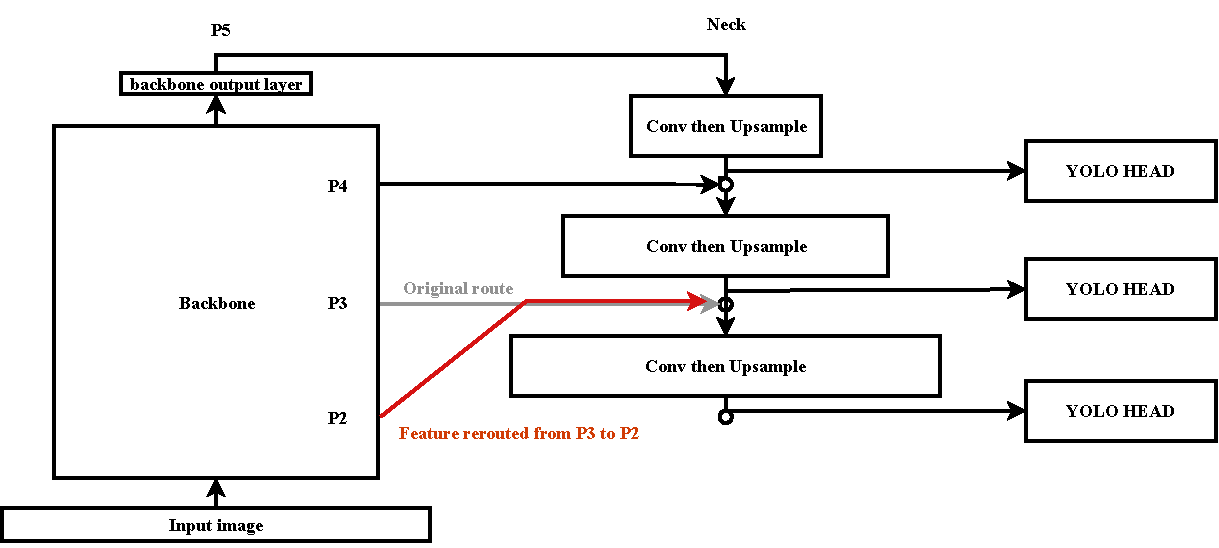
\includegraphics[width=0.4\textwidth]{../book/figures/neck-move-back.pdf}}
  %%\caption{Rerouting Neck Feature-map Source}
  %%\label{fig:neck-move-back}
  %%\end{figure}
  %%The source feature map that was fed on the feature pyramid can be rerouted 
  %%to a shallower layer of the backbone (look at Fig. \ref{fig:neck-move-back}). 
  %%By using the shallower layer, the input data will have a shorter propagation through the neural network.
  %%This way, less information will be lost through propagation layer-by-layer.

  %The shallower layer (layers that are closer to the input) has more 
  %information about the image, albeit have less abstraction. 
  %By doing this, we avoid the loss of information.
  
  \item {Additional Detection Layer}

  We add a head detection layer to the neural network, increasing from the original 3 to 4.
  %\begin{figure}[htbp]
  %\centerline{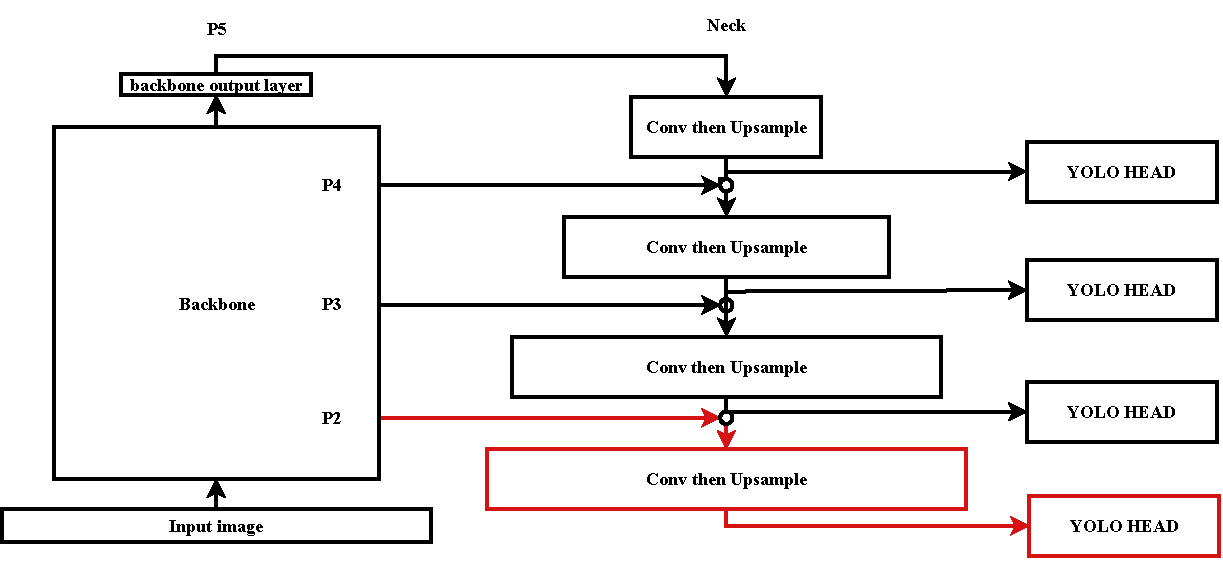
\includegraphics[width=0.4\textwidth]{../book/figures/addmorehead.pdf}}
  %\caption{Adding More Detection Layer}
  %\label{fig:add-head}
  %\end{figure}
  %An additional detection layer enable YOLOv7 to detect at more scales. With more scales,
  %the detection layers can be more specialized to specific cluster of data.
  %This approach has been tried in \cite{barunastra} by increasing the number of
  %detection layer from 2 to 3 in YOLOv4-tiny. In this experiment, we will increase
  %the number of detection layer from 3 to 4.

  \item {Replacing Detection Layer to Decoupled Anchor-Free Head}

  We replace the head layer from anchor head to decoupled anchor-free head of YOLOv6.
  %One of the advantage of anchor-free model to anchor-based model
  %is that it decreases the amount of heuristic tuning parameter as we don't
  %have to define the anchors. \cite{yolox}\cite{yolov6} reported that using anchor-free
  %head increases the accuracy and decreases the number of parameters in the model,
  %resulting in a faster and more accurate model.
  
  \item {Partitioning Image for Inference}

  We do detection by partitioning the image into 4.
  %Partitioning the image has the potential to improve the accuracy of small object detection.
  %By partitioning an image into multiple smaller images as shown in Fig. \ref{fig:partition}, 
  %the down-scaling factor of the original image to neural network input size is greatly reduced,
  %thereby reducing the loss of information. This approach allows the finer detail like small objects in the data.
  
  %One challenge with partitioning is the latency. As the neural network has to perform detection on each partition, the
  %total inference time is multiplied by the number of partitions.
\end{itemize}
\end{block}



%  %----------------------------------------------------------------------------------------
%  %	METHODS
%  %----------------------------------------------------------------------------------------
%  
%  \begin{block}{Methods}
%  
%  \begin{itemize}
%  \item Maecenas Vel Nisl Elit
%  \begin{itemize}
%  \item Suspendisse potenti. Fusce a est eget turpis rhoncus varius sed sed dui. Cras justo nibh, bibendum a cursus eget, consequat et dui. Maecenas vel nisl elit, sed dignissim dolor. 
%  \item In hac habitasse platea dictumst.
%  \end{itemize}
%  
%  \item Viewpoint Matching Constraints
%  \begin{itemize}
%  \item Cum sociis natoque penatibus et magnis dis parturient montes, nascetur ridiculus mus. 
%  \item Proin in nisi diam.
%  \item Nam ultricies pellentesque nunc, ultrices volutpat nisl ultrices a.
%  \end{itemize}
%  
%  \item Volutpat 
%  \begin{itemize}
%  \item Duis semper lorem eget dui dignissim porttitor.
%  \item Nulla facilisi. In ullamcorper lorem quis dolor.
%  \end{itemize}
%  \end{itemize}
%  
%  \end{block}
%  
%  %----------------------------------------------------------------------------------------
%  %	MATHEMATICAL SECTION
%  %----------------------------------------------------------------------------------------
%  
%  \begin{block}{Mathematical Section}
%  
%  \begin{itemize}
%  \item Maecenas Ultricies Feugiat Velit Non Mattis.
%  \begin{itemize}
%  \item Duis ante erat, bibendum nec tempus nec, interdum quis est. Nulla at mollis tortor. Phasellus quis leo dolor, aliquam laoreet orci $X$ Donec dapibus sagittis neque eu nec, interdum quis est. $Y_n, n=1,\cdots,N$ ndum nec tempus nec, interd
%  \begin{align*}
%  X \rightarrow r(X) & = \arg \max_{c} \Big\{ \max_n \big\{ \sum_{x_i \in X} \delta(x_i,Y_{n,c})\big\} \Big\} 
%  \end{align*}
%  \item Cras faucibus scelerisque cursus. Proin ut vestibulum augue. $\delta(x_i,Y_{n,c})$
%  \end{itemize}
%  \item Fusce tempus arcu id ligula varius dictum. Donec ut nisl dui, ac consectetur elit. In nec enim porta augue venenatis sollicitudin. Phasellus quis nunc neque. Suspendisse mauris diam, suscipit non gravida in, placerat id enim. Ut nec ipsum in lectus ultrices sagittis.
%  \end{itemize}
%  
%  \end{block}
%  
%  %----------------------------------------------------------------------------------------

\end{column} % End of the first column

\begin{column}{.03\textwidth}\end{column} % Empty spacer column
 
\begin{column}{.465\textwidth} % The second column

%----------------------------------------------------------------------------------------
%	RESULTS
%----------------------------------------------------------------------------------------
%\begin{block}{Methodology: Step by Step}
%  To conduct this study, first the dataset must be prepared to conform with format understandable by YOLOv7.
%  Then, to aid and accelerate the process of this study, we will automate the training process.
%  Modification configurations will be made and then inputted to the trainer. 
%  These modifications might or might not include a combinations of modifications candidates.
%  The trainer will built neural network according to the modification configuration and train them.
%  The traned neural networks will be analyzed for their performance and to look for potential modifications that can be made to optimize the neural network more.
%  If such modification was found, we will create a configuration for it and then feed it to the trainer.
%  Finally, among all of the modifications, the best model will be chosen.
%  The best model will be decided according to their mAP score.
%\end{block}


%\begin{block}{Modifications Candidates}
%  \begin{itemize}
%    \item Bag-of-Freebies Modifications
%    \begin{itemize}
%      \item On-training Anchor Box Recalculation
%      A layer will be added in the neural network to learn the optimal size
%      for anchor box. 
%      In most YOLO architectures, the anchor box are constant and calculated prior to training.
%      \item Mosaic Augmentation
%      Mosaic Augmentations has been proven to increase the object detection accuracy in YOLOv4 and YOLOv5.
%    \end{itemize}
%    \item Architecture Modifications
%    \begin{itemize}
%      \item Neck Modifications
%      Some layer of the neck will be modified to take input from a more shallow layer of the backbone of YOLOv7.
%      \item Head layer addition
%      Another head layer will be added so that YOLOv7 can detect on a higher scale.
%    \end{itemize}
%  \end{itemize}
%\end{block}

\begin{block}{Result}
\begin{itemize}
  \item Mosaic Augmentation and Anchor Recalculation
    \begin{table}
    \small
      \begin{tabular}{ l l c }
    \toprule[1.5pt]
    No & Model        &mAP@50 \\
    \midrule
    0  & \texttt{YOLOv7-plain}        & 0\%\\
    1  & \texttt{YOLOv7-M}            & 0\%\\
    2  & \texttt{YOLOv7-AR}           & 0\%\\
    3  & \texttt{\textbf{YOLOv7-MAR}} & \textbf{11.2}\%\\
    \midrule
       & Improvement                  & \textbf{\textcolor{green}{+11.2\%}}\\
    \bottomrule[1.5pt]
  \end{tabular}
    \end{table}
  \item EIoU Localization Loss
    \begin{table}
    \small
      \begin{tabular}{ l l c }
    \toprule[1.5pt]
    No & Modification        &mAP@50 \\
    \midrule
    0  & \texttt{\textbf{YOLOv7-MAR +CIoU}} (original)     & \textbf{11.2}\%\\
    1  & \texttt{YOLOv7-MAR + EIoU}                & 0\%\\
    2  & \texttt{YOLOv7-MAR + EIoU + Convexication} & 4.92\%\\
    \midrule
       & Peningkatan                                & \textbf{\textcolor{red}{-6.28\%}}\\
    \bottomrule[1.5pt]
  \end{tabular}
    \end{table}
  \item {Reroute Neck Feature-map Source}
    \begin{table}
    \small
      \begin{tabular}{ l l c }
    \toprule[1.5pt]
    No & Modification                                      &mAP@50 \\
    \midrule
    0  & \texttt{YOLOv7-MAR}                           & 11.2\%\\
    1  & \texttt{\textbf{YOLOv7-MAR + rerouting}} & \textbf{14.09\%}\\
    \midrule
       & Improvement                                & \textbf{\textcolor{green}{+2.98\%}}\\
    \bottomrule[1.5pt]
  \end{tabular}
    \end{table}
  \item {Additional Detection Layer}
    \begin{table}
    \small
      \begin{tabular}{ l l c }
    \toprule[1.5pt]
    No & Modifikasi                                 &mAP@50 \\
    \midrule
    0  & \texttt{YOLOv7-MAR}                        & \textbf{11.2\%}\\
    1  & \texttt{YOLOv7-MAR + more head}            & 5.19\%\\
    \midrule
       & Improvement                                & \textbf{\textcolor{red}{-6\%}}\\
    \bottomrule[1.5pt]
  \end{tabular}
    \end{table}
  \item {Replacing Detection Layer to Decoupled Anchor-Free Head}
    \begin{table}
    \small
    \begin{tabular}{ l l c }
  \toprule[1.5pt]
  No & Model                                 &mAP@50 \\
  \midrule
  0  & \texttt{YOLOv7-MAR (anchor head)}        & \textbf{11.2\%}\\
  1  & \texttt{YOLOv7-MAR + anchor-free head}       & 0\% Bug Fix Data Coming Up\\
  \bottomrule[1.5pt]
\end{tabular}
    \end{table}
  \item {Partitioning Image for Inference}
    \begin{table}
    \small
    \begin{tabular}{ l l c c c}
  \toprule[1.5pt]
  No & Model                                       &  Input Size  &Partition4 mAP@50               &mAP@50\\
  \midrule
  0  & \texttt{YOLOv7-AR}                          &     960      & 2.9\%                          &TBA\\
  1  & \texttt{YOLOv7-MAR}                         &     640      & 18.46\%                        &TBA\\
  3  & \texttt{YOLOv7-MAR}                         &     960      & 37.69\%                        &TBA\\
  4  & \texttt{YOLOv7-MAR + rerouting}             &     960      & 30.04\%                        &TBA\\
  5  & \texttt{YOLOv7-MAR + more head}             &     960      & 10.53\%                        &TBA\\
  6  & \texttt{YOLOv7-MAR + anchor-free}           &     640      & 37.57\%                        &TBA\\
  7  & \texttt{\textbf{YOLOv7-MAR + anchor-free}}  &     960      &\textbf{46.18\%}                &TBA\\
  %\midrule
  %   & Improvement                                 &              & \textbf{\textcolor{red}{-6\%}} &TBA\\
  \bottomrule[1.5pt]
\end{tabular}
    \end{table}
\end{itemize}

From the result, we can conclude that using anchor-free head with mosaic augmentation and partitioning, we can produce the greatest mAP score of 46.18\%.
\end{block}

%------------------------------------------------

% %----------------------------------------------------------------------------------------
% %	ACKNOWLEDGEMENTS
% %----------------------------------------------------------------------------------------
% 
% \begin{block}{Acknowledgments}
% 
% \begin{itemize}
% \item Nam mollis tristique neque eu luctus. Suspendisse rutrum congue nisi sed convallis. Aenean id neque dolor. Pellentesque habitant morbi tristique senectus et netus et malesuada fames ac turpis egestas.
% \end{itemize}
% 
% \end{block}
% 
% %----------------------------------------------------------------------------------------
% %	CONTACT INFORMATION
% %----------------------------------------------------------------------------------------
% 
%\setbeamercolor{block title}{fg=black,bg=orange!70} % Change the block title color
%
%\begin{block}{Contact Information}
%
%\begin{itemize}
%\item Implementation: \href{https://github.com/messier12/final-project-yolo-optimization.git}{https://github.com/messier12/final-project-yolo-optimization.git}
%\item Email: \href{mailto:solang.dion@gmail.com}{solang.dion@gmail.com}
%\item Phone: +62 813 2752 2023
%\end{itemize}
%
%\end{block}

%----------------------------------------------------------------------------------------

\end{column} % End of the second column

\begin{column}{.015\textwidth}\end{column} % Empty spacer column

\end{columns} % End of all the columns in the poster

\end{frame} % End of the enclosing frame

\end{document}